\section{Domain Model}
    \begin{figure}[H]
        \centering
        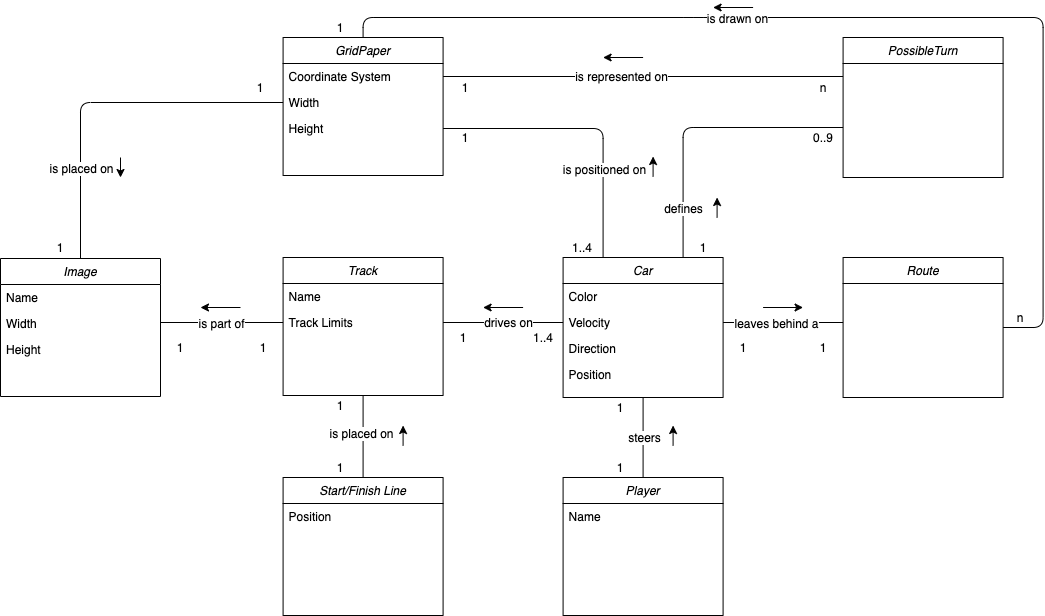
\includegraphics[width=18cm,keepaspectratio,center]{img/Domain-Model.png}
        \caption{Domain Model of RaceTrack}
    \end{figure}

    The \textit{\gls{Track}}, with a \textit{\gls{Start/Finish Line}} placed on it, is part of an \textit{\gls{Image}}. In the end, a \textit{\gls{GridPaper}} is placed on the image, which defines the points players can drive to. There are between one and four cars that drive on the \textit{Track}, they are placed on the \textit{\gls{Start/Finish Line}} before the game starts. Each \textit{\gls{Car}} is being steered by a \textit{\gls{Player}}. A \textit{Car} is always being positioned on the \textit{GridPaper}. The \textit{Car} defines its \textit{\gls{PossibleTurn}} through his velocity and direction. Each \textit{PossibleTurn} is represented on the \textit{GridPaper} itself. While driving, the \textit{Car} leaves behind a \textit{\gls{Route}}, which is also drawn on the \textit{GridPaper}.